\lab{Anisotropic Diffusion}{Anisotropic Diffusion}
\label{lab:AnisotropicDiffusion}

\objective{Demonstrate the use of finite difference schemes in image analysis.}

We will now look into one of the many applications of finite difference methods.
It is often useful in image processing to remove extra static from an image.
This is most easily done by simply blurring the image, but this has the unfortunate consequence of also blurring the boundary lines between distinct elements of the image.
This blurring can be done by treating the image as a rectangular domain where we are applying the diffusion equation:
\[u_t = b \Delta u\]
where $b$ is some diffusion constant and $\Delta$ is the Laplace operator.
In this simple case, the diffusion equation is the same as the heat equation.
A more general form of the diffusion equation in two dimensions is:
\[u_t = \nabla\cdot \left( c(x,y,t) \nabla u \right)\]
where $c$ is a function representing the diffusion coefficient at each given point and time.
In this case, $\nabla \cdot$ is the divergence operator and $\nabla$ is the gradient. 
If we want to blur a picture uniformly, we can allow $c$ to be constant, but we are often interested in \textit{preserving the edges} between features of the image.
$c$ can be used to control how much diffusion is allowed at each point, so we would like to modify it so that it minimizes diffusion across edges in the image.
If we can limit diffusion near the boundaries between different features of the image, we will be able to allow smaller details of the image to blur away while maintaining the overall form of the image.
This is especially useful for denoising low quality images.
This approach was first introduced by Pietro Perona and Jitendra Malik in 1987.
It is known as Anisotropic Diffusion or Perona-Malik Diffusion.

Suppose we have some estimate $E$ of the rate of change at a given point in an image.
This means that $E$ will be large at boundaries in the image and small elsewhere.
We will then let $c(x,y,t) = g(E(x,y,t))$ where $g$ is some function such that $g(0)=1$ and $\displaystyle{\lim_{x \to \infty} g(x) = 0}$.
The idea here is that $c$ will be small where $E$ is large, so there will be little diffusion near the boundaries of different portions of the image.

One way to model the evolution of this system is to use a finite differencing scheme where, at each time step, we have an array of values at a 2D grid of points.
Here we will let $U_{l,m}^n$ be our discretized approximation of the function $u$, $n$ be the index in time, $l$ be the index along the $x$-axis, and $m$ be the index along the $y$-axis.

We will implement this idea of limiting diffusion at edges in the following way:
The following finite difference scheme is consistent with the Laplace Operator:
\[\Delta u = u_{xx}+u_{yy} \approx \frac{U_{l-1,m}^n - 2 U_{l,m}^n + U_{l+1,m}^n}{(\Delta x)^2} + \frac{U_{l,m-1}^n-2 U_{l,m}^n + U_{l,m+1}^n}{(\Delta y)^2}\]
Since we are working with images, we may say, without loss of generality, that the distance between pixels is always one, so $\Delta x = \Delta y = 1$. Rearranging the terms we have:
\[\Delta u \approx (U_{l-1,m}^n - U_{l,m}^n) + (U_{l+1,m}^n - U_{l,m}^n) + (U_{l,m-1}^n - U_{l,m}^n) + (U_{l,m+1}^n - U_{l,m}^n)\]

Again, since we are working with images and not some time based problem, we may say, without loss of generality, that $\Delta t = 1$, so we will have the following finite difference scheme:
\[U_{l,m}^{n+1} = U_{l,m}^n + (U_{l-1,m}^n - U_{l,m}^n) + (U_{l+1,m}^n - U_{l,m}^n) + (U_{l,m-1}^n - U_{l,m}^n) + (U_{l,m+1}^n - U_{l,m}^n)\]
We will now limit the diffusion near the edges of objects by making the following modification:
\begin{align*}
U_{l,m}^{n+1} = U_{l,m}^n + & \lambda (g(|U_{l-1,m}^n - U_{l,m}^n|)(U_{l-1,m}^n - U_{l,m}^n) \\
			&+ g(|U_{l+1,m}^n - U_{l,m}^n|)(U_{l+1,m}^n - U_{l,m}^n) \\
			&+ g(|U_{l,m-1}^n - U_{l,m}^n|)(U_{l,m-1}^n - U_{l,m}^n) \\
			&+ g(|U_{l,m+1}^n - U_{l,m}^n|)(U_{l,m+1}^n - U_{l,m}^n))
\end{align*}

Where $\lambda \leq \frac{1}{4}$ for stability.

In this way, we allow each term to be affected most by the terms that are already the most similar to it, so less diffusion will happen anywhere where there is a sharp difference between pixels.

This particular scheme has the useful property that it does not increase or decrease the total brightness of the image.
Intuitively, this is because the effect of each point on each of its neighbors is exactly opposite the effect its neighbors have on it.

Two good examples of commonly used functions for $g$ are $g(x) = e^{-\left(\frac{x}{\sigma}\right)^2}$ and $g(x) = \frac{1}{1+\left(\frac{x}{\sigma}\right)^2}$.
In both cases, $\sigma$ is a parameter which allows us to control how sharply we decrease diffusion across boundaries.
Larger $\sigma$ values allow more diffusion across boundaries.
Also note that in both cases, $g(0) = 1$ and $\displaystyle{\lim_{x\to \infty} g(x) = 0}$.
For our examples here we use $g(x)=e^{-\left(\frac{x}{\sigma}\right)^2}$.

It is worth noting that this particular difference scheme is \textit{not} an accurate finite difference scheme for the version of the diffusion equation we discussed before, but it \textit{does} accomplish the same thing in the same way.
As it turns out, this particular scheme is the solution to a slightly different diffusion PDE, but can still be used the same way.

For all of the examples here we have read in the image using the \li{scipy.misc.imread} function, and normalized it so that the colors are represented as floating point values between 0 and 1.
An image can converted to black and white when it is read by including the argument \li{flatten=True}

We can implement the above finite difference scheme using purely vector operations.
First consider the case where the boundaries of the image are considered fixed.
A simple idea would be to do the following
\begin{lstlisting}
import numpy as np
from scipy.misc import imread, imsave
from matplotlib import pyplot as plt
from matplotlib import cm

def anisdiff_bw_noBCs(U, N, lambda_, g):
    """ Run the Anisotropic Diffusion differencing scheme
    on the array A of grayscale values for an image.
    Perform N iterations, use the function g
    to limit diffusion across boundaries in the image.
    Operate on A inplace. """
    for i in xrange(N):
        U[1:-1,1:-1] += lambda_ * \
                        (g(U[:-2,1:-1] - U[1:-1,1:-1]) *
                          (U[:-2,1:-1] - U[1:-1,1:-1]) +
                         g(U[2:,1:-1] - U[1:-1,1:-1]) *
                          (U[2:,1:-1] - U[1:-1,1:-1]) +
                         g(U[1:-1,:-2] - U[1:-1,1:-1]) *
                          (U[1:-1,:-2] - U[1:-1,1:-1]) +
                         g(U[1:-1,2:] - U[1:-1,1:-1]) *
                          (U[1:-1,2:] - U[1:-1,1:-1]))
\end{lstlisting}
We can use this code on an image like this:
\begin{lstlisting}
from scipy.misc import imread, imsave
from matplotlib import pyplot as plt
from matplotlib import cm

# Read the image file 'test.png'.
# Multiply by 1. / 255 to change the values so that they are floating point
# numbers ranging from 0 to 1.
U = imread('test.jpg', flatten=True) * (1. / 255)
# Set inputs for the function.
sigma = .1
g = lambda x: np.exp(x * x * (-1. / sigma**2))
lambda_ = .25
N = 50
anisdiff_bw_noBCs(U, N, lambda_, g)
# Show the image.
plt.imshow(U, cmap=cm.gray)
plt.show()
\end{lstlisting}

Unfortunately, with reasonably sized images, this is still slow.
This happens for a variety of reasons.
When evaluating such a large vector expression, many temporary arrays are allocated and deallocated at each time step.
As you can also see, there are many repeated computations.
We do not need to calculate the differences between each point and the one next to it twice as we are doing here.
We could also take advantage of the fact that the difference between values at each point is usually (except at the boundaries) used twice in two different terms.
Each difference between pixels is used in the computations involving both of those pixels, once to find the right value of $g$ and once when we multiply by the value of $g$.
To optimize these operations we could precompute the differences in each direction and use them more intelligently.
The last issue is that, in performing these operations the way we do, we are not iterating over memory efficiently.
To compute the value of this expression, the computer also must iterate many times over different blocks of memory.
That also slows things down.

Though this code is moderately fast, it is an example where NumPy operations with slicing are not quite enough.
A partial solution would be to implement the same algorithm without using expressions that allocate temporary arrays.
The best way to do this is with inplace operations.
That will ensure that our code is not being slowed down by the costs from allocating and deallocating temporary arrays.
We can also work to eliminate all duplicate computations in our difference scheme.
Doing so gives us the following implementation of the same algorithm.
Note! This is still not the simplest way to do this, but these are the sorts of operations that a student will want to understand to be able to code this algorithm well.
\begin{lstlisting}
def anisdiff_bw_noBCs_fast(U, N, lambda_, sigma):
    """ Run the Anisotropic Diffusion differencing scheme
    on the array U of grayscale values for an image.
    Perform N iterations, use the function g = e^{-x^2/sigma^2}
    to limit diffusion across boundaries in the image.
    Operate on U inplace. """
    # Make an array to store temporary values.
    # Here we'll use reshaped versions of it in two different cases.
    diff_base = np.empty(max(U[1:,1:-1].size, U[1:-1,1:].size))
    # Make the two different reshaped versions we'll be using.
    # One to hold the differences between pixels that are adjacent vertically.
    # One to hold the differences between pixels that are adjacent horizontally.
    vdifs = diff_base[:U[1:,1:-1].size].reshape(U[1:,1:-1].shape)
    hdifs = diff_base[:U[1:-1,1:].size].reshape(U[1:-1,1:].shape)
    # Do the same thing to get temporary arrays to store the values of g.
    gvals = np.empty(max(vdifs.size, hdifs.size))
    vg = gvals[:vdifs.size].reshape(vdifs.shape)
    hg = gvals[:hdifs.size].reshape(hdifs.shape)
    # Make another array to store what we are adding to each pixel.
    # In this case, since the boundaries are fixed, we really only need to
    # store the changes to the center.
    differences = np.empty_like(U[1:-1,1:-1])
    # Store this constant to do floating point multiplication across an array
    # instead of floating point division.
    c = -1. / sigma**2
    for i in xrange(N):
        # First do all the computations involving the virtical differences.
        # Copy the values of the lower portion of A into vdifs.
        vdifs[:] = U[:-1,1:-1]
        # Compute the differences in place.
        vdifs -= U[1:,1:-1]
        # Copy the differences into vg.
        vg[:] = vdifs
        # Square them in place.
        vg *= vg
        # Multiply in place by -1. / sigma**2.
        vg *= c
        # Take the exponential function in place.
        np.exp(vg, out=vg)
        # Multiply by vdifs in place to get the portion
        # that will be added or subtracted from each pixel.
        vg *= vdifs
        # Add the values in to the differences array.
        # In this case, since the differences array is
        # uninitialized, the first operation is just a copy.
        # This accounts for the difference between each point
        # and the one above it.
        differences[:] = vg[:-1]
        # This accounts for the difference between each point
        # and the one below it.
        differences -= vg[1:]
        # Now do all the computations involving the horizontal differences.
        # Copy the values of the left portion of A into hdifs.
        hdifs[:] = U[1:-1,:-1]
        # Compute the differences in place.
        hdifs -= U[1:-1,1:]
        # Copy the differences into hg.
        hg[:] = hdifs
        # Square them in place.
        hg *= hdifs
        # Multiply in place by -1. / sigma**2.
        hg *= c
        # Take the exponential function in place.
        np.exp(hg, out=hg)
        # Multiply by hdifs in place to get the portion
        # that will be added or subtracted from each pixel.
        hg *= hdifs
        # Add the values in to the differences array.
        # This accounts for the difference between each point
        # and the one to its left.
        differences += hg[:,:-1]
        # This accounts for the difference between each point
        # and the one to its right.
        differences -= hg[:,1:]
        # Now multiply the sum of all the different terms by lambda_.
        differences *= lambda_
        # Add the differences to A in place to update its values.
        U[1:-1,1:-1] += differences
\end{lstlisting}
This is significantly faster, but much more messy.
Unfortunately, there is still a significant speed loss from iterating over the arrays many more times than is actually necessary when performing computation.
There is still a good way to address this problem.
We can use the package numexpr to perform multiple computations on an array all at once.
Numexpr is a package that can evaluate simple algebraic expressions involving arrays quickly by recognizing and computing common subexpressions and optimizing for fast cache management when accessing memory.
You may recall that the primary function in the user interface of numexpr is the \li{evaluate} function.
It evaluates an expression (in some cases, much faster than NumPy can) that has been expressed as a string containing the names of array objects that are in the current scope.
Here is how this same algorithm can be written using numexpr.
\begin{lstlisting}
import numexpr as ne
def anisdiff_bw_noBCs_numexpr(U, N, lambda_, sigma):
    """ Run the Anisotropic Diffusion differencing scheme
    on the array U of grayscale values for an image.
    Perform N iterations, use the function g = e^{-x/sigma}
    to limit diffusion across boundaries in the image.
    Operate on U inplace. U is expected to be an array
    of 32 bit floating point numbers. """
    # numexpr needs numpy float32 objects to use as a constants.
    # Start by making them.
    sinv = np.float32(-1. / sigma**2)
    l32 = np.float32(lambda_)
    # Make a copy of U to use for updates.
    Unew = U.copy()
    # Store the different slices we need to use.
    North = U[:-1,1:-1]
    South = U[1:,1:-1]
    West = U[1:-1,:-1]
    East = U[1:-1,1:]
    # Store the slice we need to use in Unew.
    newCenter = Unew[1:-1,1:-1]
    # Make various temporary arrays.
    temp = np.empty_like(U)
    vtemp = temp[:-1,1:-1]
    vtemp_upper = vtemp[:-1]
    vtemp_lower = vtemp[1:]
    htemp = temp[1:-1,:-1]
    htemp_left = htemp[:,:-1]
    htemp_right = htemp[:,1:]
    for i in xrange(N):
        # Use numexpr to compute the values to add or subtract from each pixel
        # corresponding to the differences between pixels in the up-down direction.
        ne.evaluate('l32 * exp(sinv * (South - North)**2) * (South - North)', out=vtemp)
        # Add these terms to the new array of values.
        # Account for the difference between each pixel and the one above it.
        ne.evaluate('newCenter - vtemp_upper', out=newCenter)
        # Account for the difference between each pixel and the one below it.
        ne.evaluate('newCenter + vtemp_lower', out=newCenter)
        # Do the same computation for the right-left differences.
        ne.evaluate('l32 * exp(sinv * (East - West)**2) * (East - West)', out=htemp)
        # Account for the difference between each pixel and the one to its left.
        ne.evaluate('newCenter - htemp_left', out=newCenter)
        # Account for the difference between each pixel and the one to its right.
        ne.evaluate('newCenter + htemp_right', out=newCenter)
        # Copy the values into the array U to update it.
        U[:] = Unew
\end{lstlisting}
This is both cleaner and faster than our previous solution.
It allows us to perform whole groups of operations together without having to iterate through memory over and over again.
It also optimizes for cache access so that memory bandwidth is best used.

% Old problem that asked them to implement the problem without BC's.
% Hopefully giving them the code for the case without BC's will make it easier for them.
\begin{comment}
\begin{problem}
Implement the above finite difference scheme for black and white images.
Leave the boundaries constant this time and just iterate over the interior of the image.
You may use either of the two functions listed for $g$.
One possible way to do these problems is to iterate over the array and operate in place.
\end{problem}
\end{comment}

\begin{problem}
\label{prob:anisdiff_bw}
Implement an optimized version of anisotropic diffusion for black and white images using the following boundary conditions:

For the top edge let
\begin{align*}
U_{l,m}^{n+1} = U_{l,m}^n + & \lambda (g(|U_{l-1,m}^n - U_{l,m}^n|)(U_{l-1,m}^n - U_{l,m}^n) \\
					& + g(|U_{l+1,m}^n - U_{l,m}^n|)(U_{l+1,m}^n - U_{l,m}^n) \\
					& + g(|U_{l,m+1}^n - U_{l,m}^n|)(U_{l,m+1}^n - U_{l,m}^n))
\end{align*}
Do the other edges similarly.

For the top left corner let
\begin{align*}
U_{l,m}^{n+1} = U_{l,m}^n + & \lambda (g(|U_{l+1,m}^n - U_{l,m}^n|)(U_{l+1,m}^n - U_{l,m}^n) \\
					& + g(|U_{l,m+1}^n - U_{l,m}^n|)(U_{l,m+1}^n - U_{l,m}^n))
\end{align*}
Do the other corners similarly.

Essentially we are just using the terms of the difference scheme that are actually defined.

You can do this by modifying the the numexpr version already given so that it includes the boundary values in the image.
Make the following modifications to the code given above:
\begin{itemize}

\item Change the North, South, East, and West slices so that they include the boundaries.
For example, the North variable should now include all but the last row of \li{U}.

\item Define similar North, South, East and West slices for \li{Unew}.

\item Remove the variables \li{newCenter}, \li{vtemp_upper}, \li{vtemp_lower}, \li{htemp_left}, and \li{htemp_right} since they will no longer be necessary.

\item Rewrite the strings passed to the \li{evaluate} function inside the for loop to match the new slices.
The operations in place on \li{new_center} should be replaced by the correct in place operations involving the North, South, East, and West slices of \li{Unew}.
The \li{vtemp} related variables will be replaced with \li{vtemp} and the \li{htemp} related variables will be replaced with \li{htemp}.

\end{itemize}

In your function, use
\[g(x) = e^{-\left(\frac{x}{\sigma}\right)^2}\]

Here is a non-optimized function that performs the desired computations for a generic function $g$.
Use it to test your optimized version.
\begin{lstlisting}
def anisdiff_bw_withBCs(U, N, lambda_, g):
    """ Run the Anisotropic Diffusion differencing scheme
    on the array U of grayscale values for an image.
    Perform N iterations, use the function g
    to limit diffusion across boundaries in the image.
    Operate on U inplace. """
    difs = np.empty_like(U)
    for i in xrange(N):
        difs[:-1] = g(U[1:] - U[:-1]) * (U[1:] - U[:-1])
        difs[-1] = 0
        difs[1:] += g(U[:-1] - U[1:]) * (U[:-1] - U[1:])
        difs[:,:-1] += g(U[:,1:] - U[:,:-1]) * (U[:,1:] - U[:,:-1])
        difs[:,1:] += g(U[:,:-1] - U[:,1:]) * (U[:,:-1] - U[:,1:])
        difs *= lambda_
        U += difs
\end{lstlisting}
\end{problem}

\newpage
\vfill
\begin{figure}[ht]
\begin{minipage}[b]{0.45\linewidth}
\centering
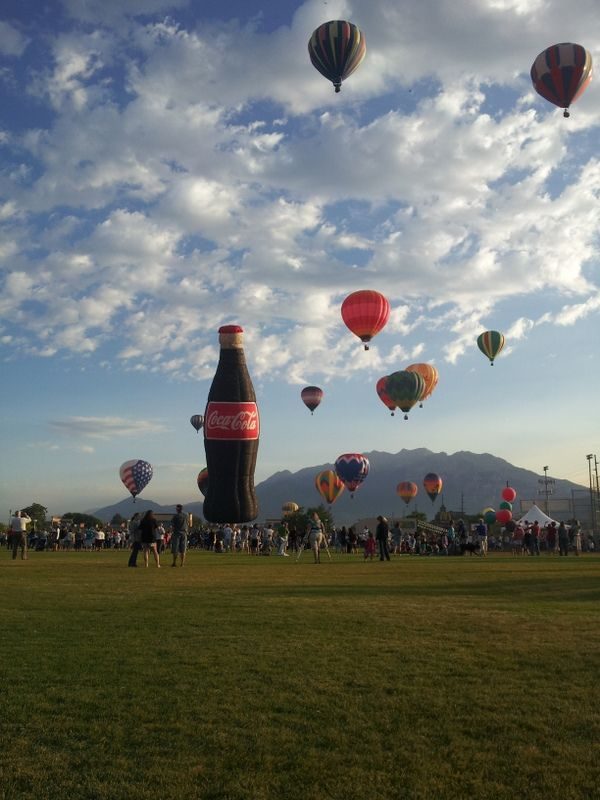
\includegraphics[width=\textwidth]{baloon_resized_color.jpg}
\caption*{original image}
\end{minipage}
\hspace{0.5cm}
\begin{minipage}[b]{0.45\linewidth}
\centering
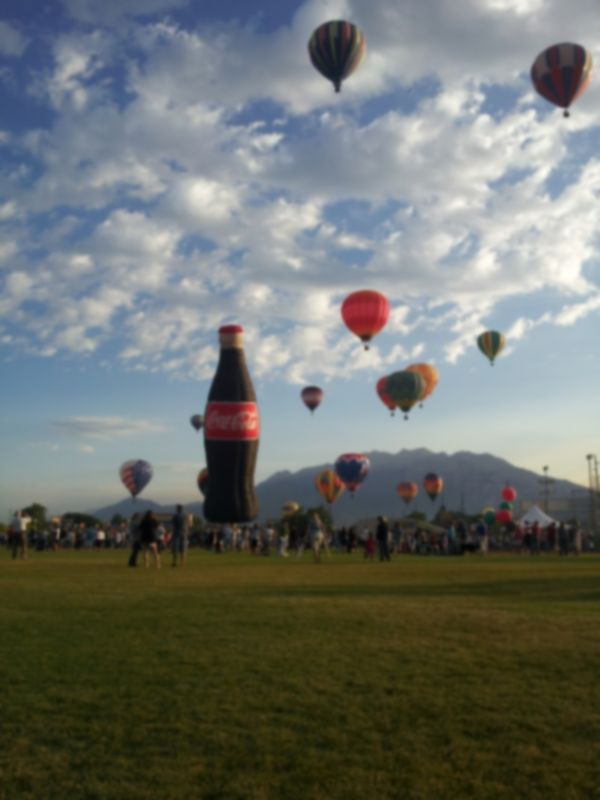
\includegraphics[width=\textwidth]{baloon_resized_color_5.jpg}
\caption*{5 iterations with $\sigma = .7$ and $\lambda = .2$}
\end{minipage}
\begin{minipage}[b]{0.45\linewidth}
\centering
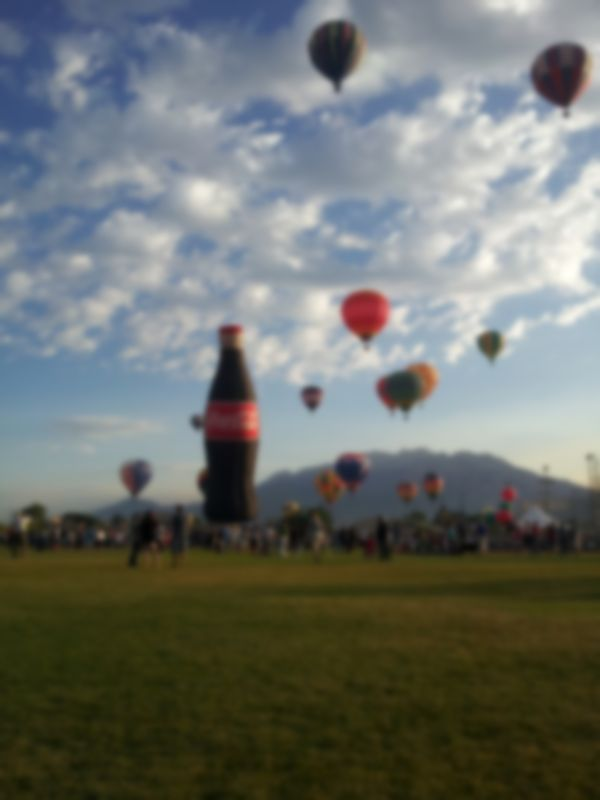
\includegraphics[width=\textwidth]{baloon_resized_color_20.jpg}
\caption*{20 iterations}
\end{minipage}
\hspace{0.5cm}
\begin{minipage}[b]{0.45\linewidth}
\centering
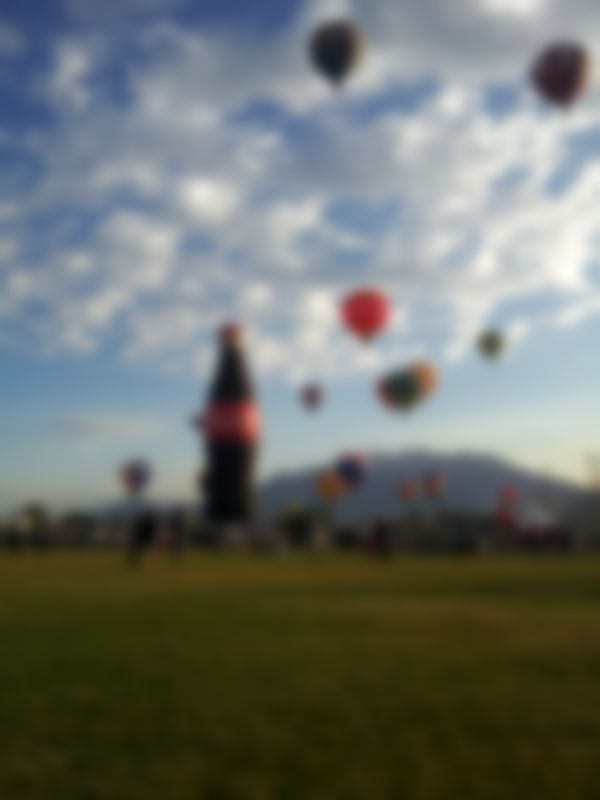
\includegraphics[width=\textwidth]{baloon_resized_color_100.jpg}
\caption*{100 iterations}
\end{minipage}
\end{figure}
\vfill
\clearpage

Colored images can be processed in a similar manner.
Instead of being represented as a two-dimensional array, colored images are represented as three dimensional arrays.
The third dimension is used to store the intensities of each of the standard 3 colors.
This diffusion process can be carried out in the exact same way, on each of the arrays of intensities for each color, but instead of detecting edges just in one color, we need to detect edges in any color, so instead of using something of the form $g(|U_{l+1,m}^n - U_{l,m}^n|)$ as before, we will now use something of the form $g(||U_{l+1,m}^n - U_{l,m}^n||)$, where $U_{l+1,m}^n$ and $U_{l,m}^n$ are vectors now instead of scalars.
The difference scheme can be treated as an equation on vectors in 3-space and now reads:
\begin{align*}
U_{l,m}^{n+1} = U_{l,m}^n + & \lambda (g(||U_{l-1,m}^n - U_{l,m}^n||)(U_{l-1,m}^n - U_{l,m}^n) \\
					& + g(||U_{l+1,m}^n - U_{l,m}^n||)(U_{l+1,m}^n - U_{l,m}^n) \\
					& + g(||U_{l,m-1}^n - U_{l,m}^n||)(U_{l,m-1}^n - U_{l,m}^n) \\
					& + g(||U_{l,m+1}^n - U_{l,m}^n||)(U_{l,m+1}^n - U_{l,m}^n))
\end{align*}

When implementing this scheme for colored images, use the $2$-norm on 3-space, i.e $||x||=\sqrt{x1^2+x2^2+x3^2}$ where $x1$, $x2$, and $x3$ are the different coordinates of $x$.

As before, this difference scheme can be implemented with simple slicing operations in NumPy.
Here is a version that solves the problem with fixed boundary conditions.
\begin{lstlisting}
def anisdiff_color_noBCs(U, N, lambda_, sigma):
    """ Run the Anisotropic Diffusion differencing scheme
    on the array A of grayscale values for an image.
    Perform N iterations, use the function g = e^{-x^2 / sigma^2}
    to limit diffusion across boundaries in the image.
    Operate on A inplace. """
    for i in xrange(N):
        U[1:-1,1:-1] += lambda_ * \
                        (np.exp((-1. / sigma**2) *
                          ((U[:-2,1:-1] - U[1:-1,1:-1])**2).sum(axis=2, keepdims=True)) *
                          (U[:-2,1:-1] - U[1:-1,1:-1]) +
                         np.exp((-1. / sigma**2) *
                          ((U[2:,1:-1] - U[1:-1,1:-1])**2).sum(axis=2, keepdims=True)) *
                          (U[2:,1:-1] - U[1:-1,1:-1]) +
                         np.exp((-1. / sigma**2) *
                          ((U[1:-1,:-2] - U[1:-1,1:-1])**2).sum(axis=2, keepdims=True)) *
                          (U[1:-1,:-2] - U[1:-1,1:-1]) +
                         np.exp((-1. / sigma**2) *
                          ((U[1:-1,2:] - U[1:-1,1:-1])**2).sum(axis=2, keepdims=True)) *
                          (U[1:-1,2:] - U[1:-1,1:-1]))
\end{lstlisting}
We can use this function like this:
\begin{lstlisting}
A = imread('test.jpg') / np.float32(255.)
Ac = A.copy()
sigma = .1
lambda_ = .2
N = 5
anisdiff_color_noBCs(A, N, lambda_, sigma)
plt.imshow(A)
plt.show()
\end{lstlisting}

As before, we can get much better performance using numexpr.
This time we must account for proper array broadcasting to be able to multiply each term by the corresponding values for $g$.
Here is how this is done in the problem with fixed boundary conditions:
\begin{lstlisting}
import numexpr as ne
def anisdiff_color_noBCs_numexpr(U, N, lambda_, sigma):
    # numexpr needs numpy float32 objects to use as a constants.
    # Start by making them.
    sinv = np.float32(-1. / sigma**2)
    l32 = np.float32(lambda_)
    # Make a copy of U to use for updates.
    Unew = U.copy()
    # Store the different slices we need to use.
    North = U[:-1,1:-1]
    South = U[1:,1:-1]
    West = U[1:-1,:-1]
    East = U[1:-1,1:]
    newCenter = Unew[1:-1,1:-1]
    # Make various temporary arrays.
    difs = np.empty_like(U)
    vdifs = difs[:-1,1:-1]
    vdifs_upper = vdifs[:-1]
    vdifs_lower = vdifs[1:]
    hdifs = difs[1:-1,:-1]
    hdifs_left = hdifs[:,:-1]
    hdifs_right = hdifs[:,1:]
    # Make an array to store the sums of the squares
    # that come when taking the norm.
    # Make 3D views of the arrays for use in broadcasting later.
    sums = np.empty(U.shape[:2], dtype=U.dtype)
    vsum = sums[:-1,1:-1]
    vsum3D = vsum[...,None]
    hsum = sums[1:-1,:-1]
    hsum3D = hsum[...,None]
    for i in xrange(N):
        # Use numexpr to compute the values to add or subtract from each pixel
        # corresponding to the differences between pixels in the up-down direction.
        # First compute the repeated values.
        ne.evaluate('South - North', out=vdifs)
        # Now compute the 2-norm squared along the last axis.
        # Store the output in vsum.
        ne.evaluate('sum(vdifs**2, axis=2)', out=vsum)
        # Now finish computing this set of terms.
        # Use the 3D view of vsum so the multiplication broadcasts
        # along the third dimension of vdifs.
        ne.evaluate('l32 * exp(sinv * vsum3D) * vdifs', out=vdifs)
        # Add these terms to the new array of values.
        # Account for the difference between each pixel and the one above it.
        ne.evaluate('newCenter - vdifs_upper', out=newCenter)
        # Account for the difference between each pixel and the one below it.
        ne.evaluate('newCenter + vdifs_lower', out=newCenter)
        # Do the same computation for the right-left differences.
        # First compute the repeated values.
        ne.evaluate('East - West', out=hdifs)
        # Now compute the 2-norm squared along the last axis.
        # Store the output in vsum.
        ne.evaluate('sum(hdifs**2, axis=2)', out=hsum)
        # Now finish computing this set of terms.
        # Use the 3D view of hsum so the multiplication broadcasts
        # along the third dimension of hdifs.
        ne.evaluate('l32 * exp(sinv * hsum3D) * hdifs', out=hdifs)
        # Account for the difference between each pixel and the one to its left.
        ne.evaluate('newCenter - hdifs_left', out=newCenter)
        # Account for the difference between each pixel and the one to its right.
        ne.evaluate('newCenter + hdifs_right', out=newCenter)
        # Copy the values into the array U to update it.
        U[:] = Unew
\end{lstlisting}

\begin{problem}
Make a new version of the code you wrote for the previous problem which processes a colored image.
Measure the difference between pixels using the $2$-norm.
Use the corresponding vector versions of the boundary conditions given in Problem \ref{prob:anisdiff_bw}.

To do this, you must break up the computation of the different terms so that you can compute the norm along each triple of color values and then broadcast the g values along the last axis of the array of differences.
This can be done by taking your code from the previous problem and doing the following:
\begin{itemize}

\item Outside the loop, define a temporary array to hold the squares of the norms of the color triples.
This should be similar to the variable \li{sums} shown in the example with fixed boundary conditions.

\item Using the array you have just allocated, make slices of it to hold the norms corresponding to the horizontal and vertical differences.
This will be like \li{hsums} and \li{vsums} in the code above.

\item Make 3D views of the arrays \li{hsums} and \li{vsums}.
There are several ways to do this.
One is shown in the example above using the \li{[...,None]} syntax.
The \li{...} says that slices that follow apply to the last axes of the array and not the first ones.
The \li{None} tells NumPy to create an array with an extra dimension of length 1 wherever the \li{None} appears.
We do this so that we can broadcast along the third axis of $U$ to multiply each value of $g$ across its corresponding color triple.

\item Split the computation of the different terms into three pieces (as shown in the example above).
Be sure to use \li{vsums} and \li{hsums} as the output arrays for the sum command and \li{vsums3D} and \li{hsums3D} to multiply the rest of the different terms by $g$.

\end{itemize}

Here is a reference implementation that you can use to verify that your optimized version is correct.
\begin{lstlisting}
def anisdiff_color_withBCs(A, N, lambda_, sigma):
    """ Run the Anisotropic Diffusion differencing scheme
    on the array A of grayscale values for an image.
    Perform N iterations, use the function g = e^{-x^2/sigma^2}
    to limit diffusion across boundaries in the image.
    Operate on A inplace. """
    sinv = -1. / sigma**2
    difs = np.empty_like(A)
    for i in xrange(N):
        difs[:-1] = np.exp(sinv * np.square(A[1:] - A[:-1]).sum(axis=2, keepdims=True)) * (A[1:] - A[:-1])
        difs[-1] = 0
        difs[1:] += np.exp(sinv * np.square(A[:-1] - A[1:]).sum(axis=2, keepdims=True)) * (A[:-1] - A[1:])
        difs[:,:-1] += np.exp(sinv * np.square(A[:,1:] - A[:,:-1]).sum(axis=2, keepdims=True)) * (A[:,1:] - A[:,:-1])
        difs[:,1:] += np.exp(sinv * np.square(A[:,:-1] - A[:,1:]).sum(axis=2, keepdims=True)) * (A[:,:-1] - A[:,1:])
        difs *= lambda_
        A += difs
\end{lstlisting}
\end{problem}

This sort of anisotropic diffusion can be very effective, but, depending on the image, it may also smear out edges that do not have large differences between them.
An example of this limitation can be seen in Figure \ref{fig:anisdif_smearing}

\begin{figure}
\begin{minipage}[b]{.45\linewidth}
\centering
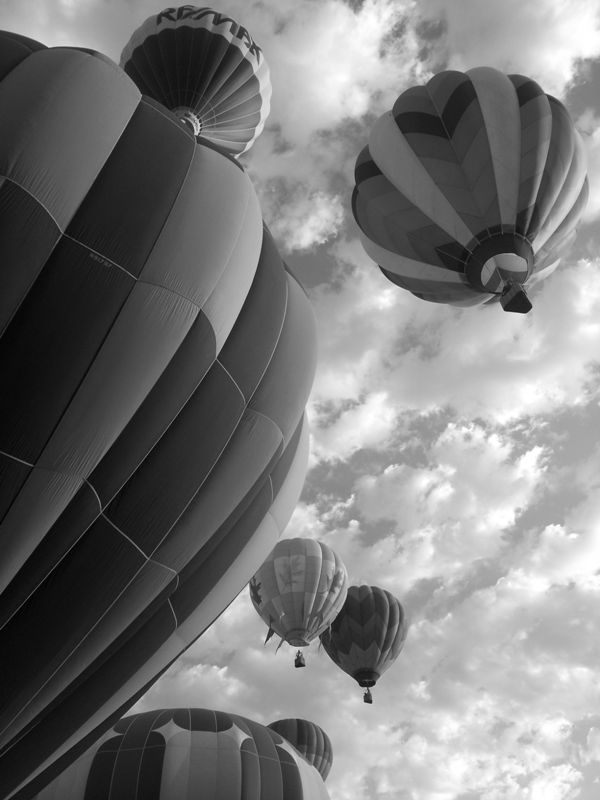
\includegraphics[width=\textwidth]{baloons_resized_bw.jpg}
\caption*{original image}
\end{minipage}
\hspace{0.5cm}
\begin{minipage}[b]{0.45\linewidth}
\centering
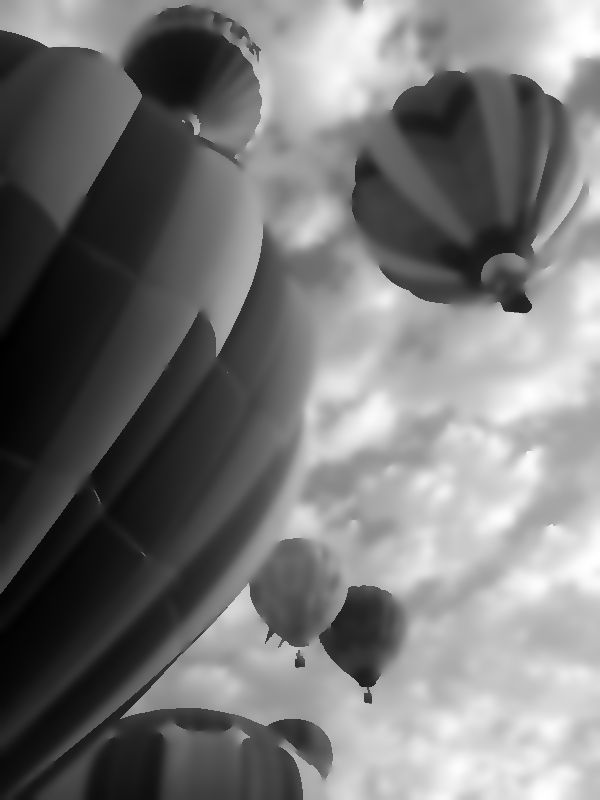
\includegraphics[width=\textwidth]{baloons_resized_bw_50.jpg}
\caption*{after 50 iterations}
\end{minipage}
\caption{Smearing of similar colors when using an anisotropic diffusion filter.}
\label{fig:anisdif_smearing}
\end{figure}

As we can see, after 100 iterations, some of the boundaries between similar shades of grey have smeared unevenly. You may still have to look closely to see it.
This can be counteracted somewhat by further decreasing the $\sigma$ value, but if we have random noise throughout the image, this will not remove it.
If we have random static in the image, we can remove this using a modified version of the filter.
Instead of measuring the rate of change in the picture in each direction, we change each point according to whether or not any of its adjacent points have roughly the same value it has.
This is called a minimum-biased filter.
This sort of trick is especially good for removing isolated pixels that are different from those around them.
A very simple way to do this is by taking the average of the two smallest differences between each pixel and its eight neighbors and using that in place of $g$ in the difference scheme above.
Along the boundaries, we do not have 8 neighbors for each pixel, but we can get by by just using the pixels we have and eliminating the other terms in the difference scheme, just as we did before.
This will make it so that points that neighbor points of similar value will not be changed, while points that do not match their surroundings will be faded to become more like the points surrounding them.
This does not have the same symmetrical diffusion as the other scheme, i.e. if one pixel changes, it does not necessarily change its neighboring pixels by the same amount.
As long as you leave $\lambda \leq \frac{1}{4}$ and you have scaled the pixels to have floating point values between 0 and 1, the scheme will still remain within its minimum and maximum bounds, since the tendency is always to move points closer to the values of their neighbors.
To demonstrate the action of such a filter, we make changes to random pixels in the color version of the same photo and use both filters to remove the noise we have added.
Below, we include an example where we have added noise to the color version of that same picture, then used a minimum-biased filter to diminish the noise and the original filter to smooth what remains.

\begin{problem}
(optional)
Implement the minimum-biased finite difference scheme described above.
\end{problem}

\newpage
\vfill
\begin{figure}[ht]
\begin{minipage}[b]{0.45\linewidth}
\centering
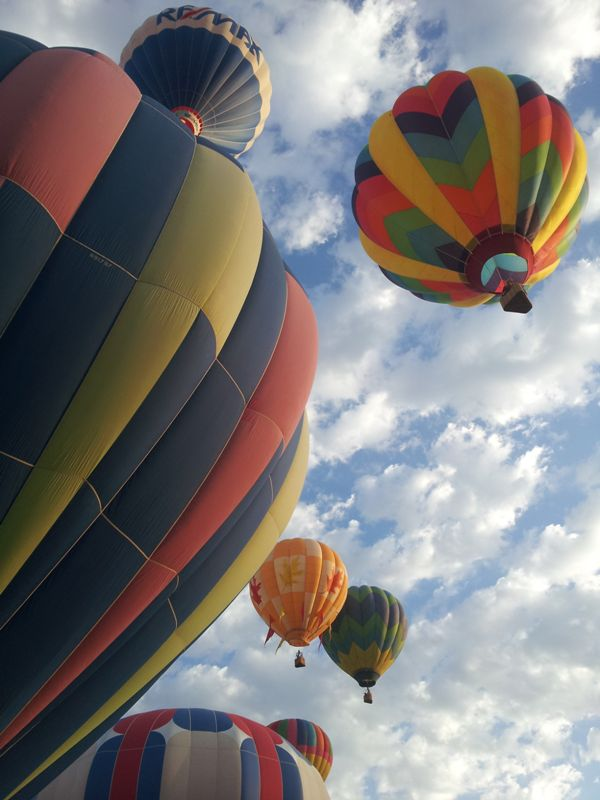
\includegraphics[width=\textwidth]{baloons_resized_color.jpg}
\caption*{original image}
\end{minipage}
\hspace{0.5cm}
\begin{minipage}[b]{0.45\linewidth}
\centering
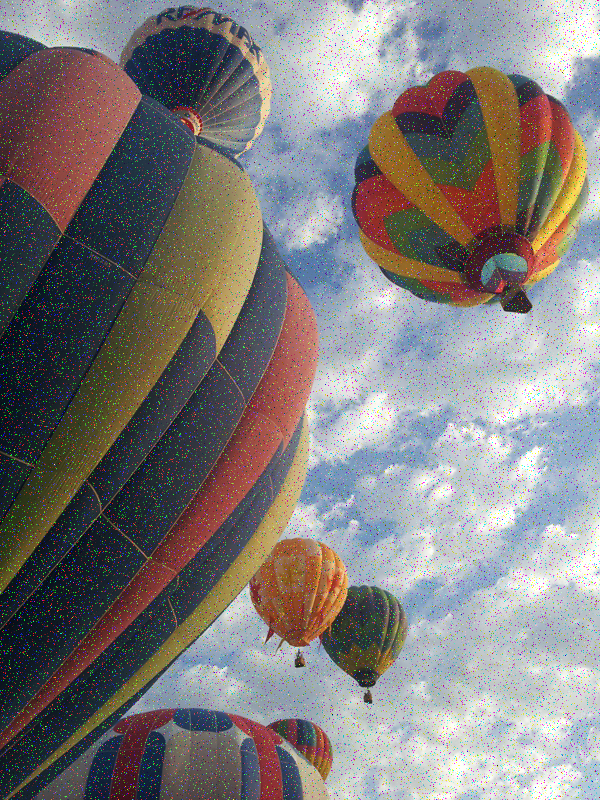
\includegraphics[width=\textwidth]{baloons_resized_noisy.png}
\caption*{randomly changed 100000 color values}
\end{minipage}
\begin{minipage}[b]{0.45\linewidth}
\centering
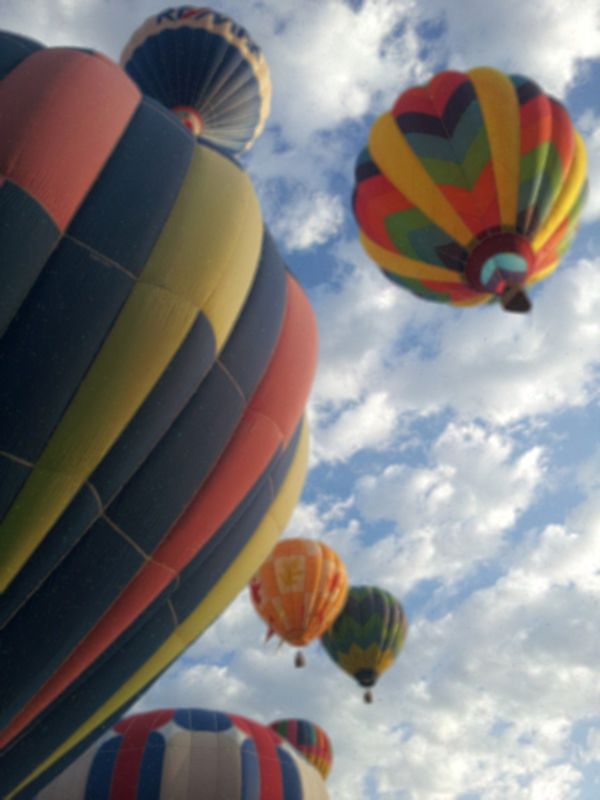
\includegraphics[width=\textwidth]{baloons_resized_minbias.jpg}
\caption*{300 iterations of a min-biased scheme}
\end{minipage}
\hspace{0.5cm}
\begin{minipage}[b]{0.45\linewidth}
\centering
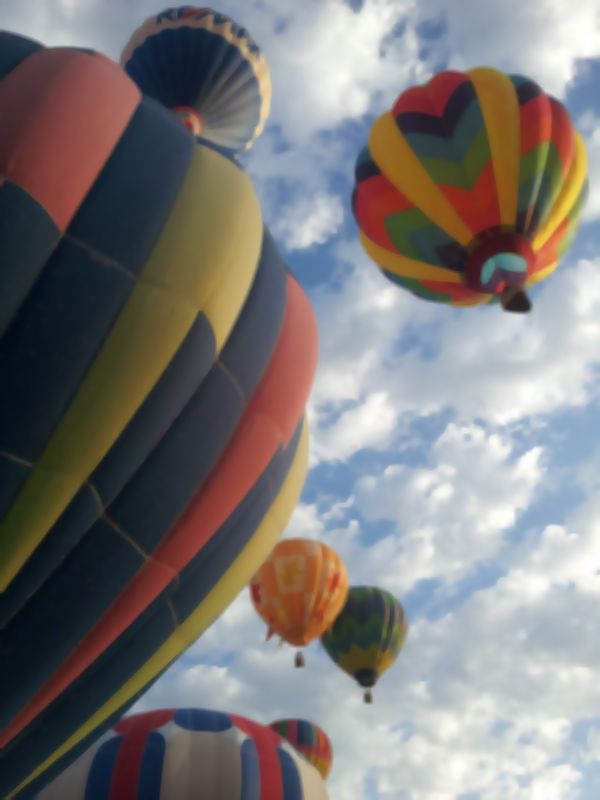
\includegraphics[width=\textwidth]{baloons_resized_both.jpg}
\caption*{after 8 additional iterations of the first filter with $\lambda=.25$ and $\sigma=.04$.}
\end{minipage}
\end{figure}
\vfill
\clearpage

\nocite{Perona1988,Kim2009}
\printbibliography 